\documentclass{standalone}
\usepackage{tikz}
\usepackage{amsmath}
\usetikzlibrary{arrows.meta, decorations.pathreplacing}

\begin{document}
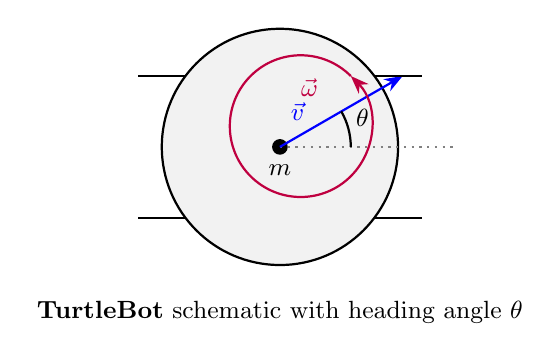
\begin{tikzpicture}[scale=1.5, every node/.style={font=\small}, >=Stealth]

  % TurtleBot body
  \draw[thick, fill=gray!10] (0,0) circle (1);
  \node[circle, fill=black, inner sep=2pt, label=below:{$m$}] at (0,0) {};

  % Reference direction (theta = 0) — dotted
  \draw[dotted, thick, gray] (0,0) -- (1.5,0);

  % Velocity vector at an angle (30 degrees)
  \draw[thick, ->, blue] (0,0) -- ({1.2*cos(30)}, {1.2*sin(30)});
  \node[text=blue] at (0.15,0.3)  {$\vec{v}$};

  % Heading angle arc and label
  \draw[thick] (0.6,0) arc[start angle=0, end angle=30, radius=0.6];
  \node at (0.7,0.25) {$\theta$};

  % Angular velocity (omega) — purple arc
  \draw[->, thick, purple] (0.6,0.6) arc[start angle=45, end angle=405, radius=0.6];
  \node[text=purple] at (0.25,0.5) {$\vec{\omega}$};

  % Wheels (spaced wider)
  \draw[thick] (-1.2,0.6) -- (-0.8,0.6);
  \draw[thick] (-1.2,-0.6) -- (-0.8,-0.6);
  \draw[thick] (0.8,0.6) -- (1.2,0.6);
  \draw[thick] (0.8,-0.6) -- (1.2,-0.6);

  % Label below
  \node at (0,-1.4) {\textbf{TurtleBot} schematic with heading angle $\theta$};

\end{tikzpicture}
\end{document}
